\chapter{Results}
\label{ch:Results}
As mentioned in the introduction, a software platform able to simulate propagation of electromagnetic waves in photonic crystals was developed. In chapter \ref{ch:Electromagnetic waves in periodic media} the equations that rule the problem where stated, and background behind one method of solution for them using FEA has been discussed in chapter \ref{ch:Finite_element_method}. In this chapter the solutions obtained by applying these concepts are presented and compared with either their analytic solutions or numerical solutions from the literature.

\section{Electrostatic benchmark tests}

Now, platform \href{https://github.com/bebopsan/peyeQM}{PeyeQM} was built in a \href{en.wikipedia.org/wiki/Top-down_and_bottom-up_design}{bottom-up } process that started by making a FE solver that could handle static scalar problems of electron confinement in 2D potential wells for application in Quantum Mechanics. This project involved an upgrade of that platform that began with the implementation of support for vector formulations, and a transition to Object Oriented Paradigm that could improve flexibility and maintenance.

The first section of this chapter shows the results obtained for Electrostatic benchmark tests, and were made in order to assert the accuracy of the static vectorial solver, and  routines for the construction of stiffness matrices.

\subsection{Electric field due to charged elements}
\subsubsection{Parallel plate capacitor}
The first experiment was to simulate the most basic field we could think of, this is, that inside a parallel plate capacitor, where field lines go straight from one plate to the other. 

Electric fields satisfy equation \ref{eq:diff_Faraday}. If there are no sources or sinks ($- \frac{\partial \mathbf{B}}{\partial t}=0)$, then the field $\mathbf{E}$ is said to be \textit{irrotational} and by an \href{http://ebooksgo.org/mathematics/Vector_Identity.pdf}{identity of vector} calculus we know that there must exist a scalar field $V$ whose gradient is a valid Electrostatic vector field:
\begin{equation}
\nabla\times\nabla V = 0
\label{eq:Laplace}
\end{equation}
Scalar equations are easier to solve and are very useful when the medium is homogeneous and isotropic, this is the reason why many books stick with scalar problems and leave the process of obtaining $\mathbf{E}$ as performing on $V$ the derivations in operator $\nabla$. Using the scalar potential as an intermediate step for the solution of $\mathbf{E}$ stops being a good idea when interfaces between mediums and sharp geometries appear, and a direct solution using vector fields gains relevance.

In a parallel plate capacitor like that in figure \ref{fig:parallel_plate}, we consider two (infinite, parallel, plane, perfectly conducting, charged) plates that occupy the planes $x = 0$ and $x = d$ kept at potentials $V = 0$ and $V = V_0$ respectively.  
With plates of very large dimensions compared to the spacing between them, the potential becomes a function of $x$ only, and equation \ref{eq:Laplace} becomes:
$$\dfrac{d^2V}{d x^2}=0$$ Integrating twice, we get: 
\begin{equation}
V(x) = Ax + B
\end{equation}
Where $A$  and $B$ are constants of integration solved by using boundary conditions.
$$V(0) = A0 + B = 0 \quad or \quad B = 0$$$$V(d) = Ad + B = V_0 \quad or \quad A = \dfrac{V_0}{d}$$

Making the particular solution for the potential:
$$V=\dfrac{V_0}{d}x \quad for \quad 0<x<d$$ 
The field is then obtained by taking the gradient of $V$, and we add a $-$ sign taking into account that $\mathbf{E}$ is a conservative field.

\begin{equation}
\mathbf{E}= -\nabla V = - \dfrac{dV}{dx}\hat{a}_x = -\dfrac{V}{d}\hat{a}_x
\end{equation}
 This means that the field is uniform and directed from the higher potential plate to the lower potential plate as shown in \ref{fig:parallel_plate} \ref{Rao2004}.

\begin{figure}
\centering
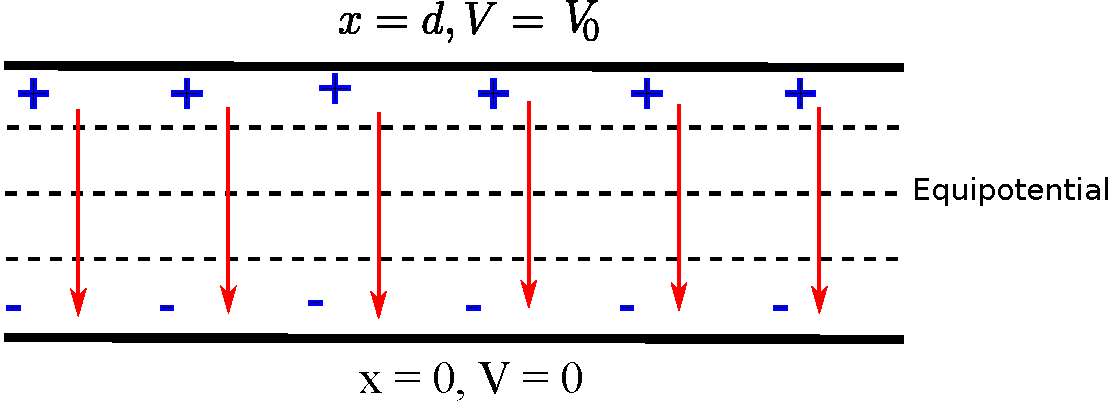
\includegraphics[scale=0.5]{./img/parallel_plate_capacitor.pdf}
\caption{Cross sectional view of parallel plate capacitor.}
\label{fig:parallel_plate}
\end{figure}

A rectangular region was meshed and Dirichlet boundary condition were applied in the bottom and top plates as a field pointing down. Separation $d$ is taken unitary and the result is shown in figure \ref{fig:capacitor}.

\begin{figure}
\centering
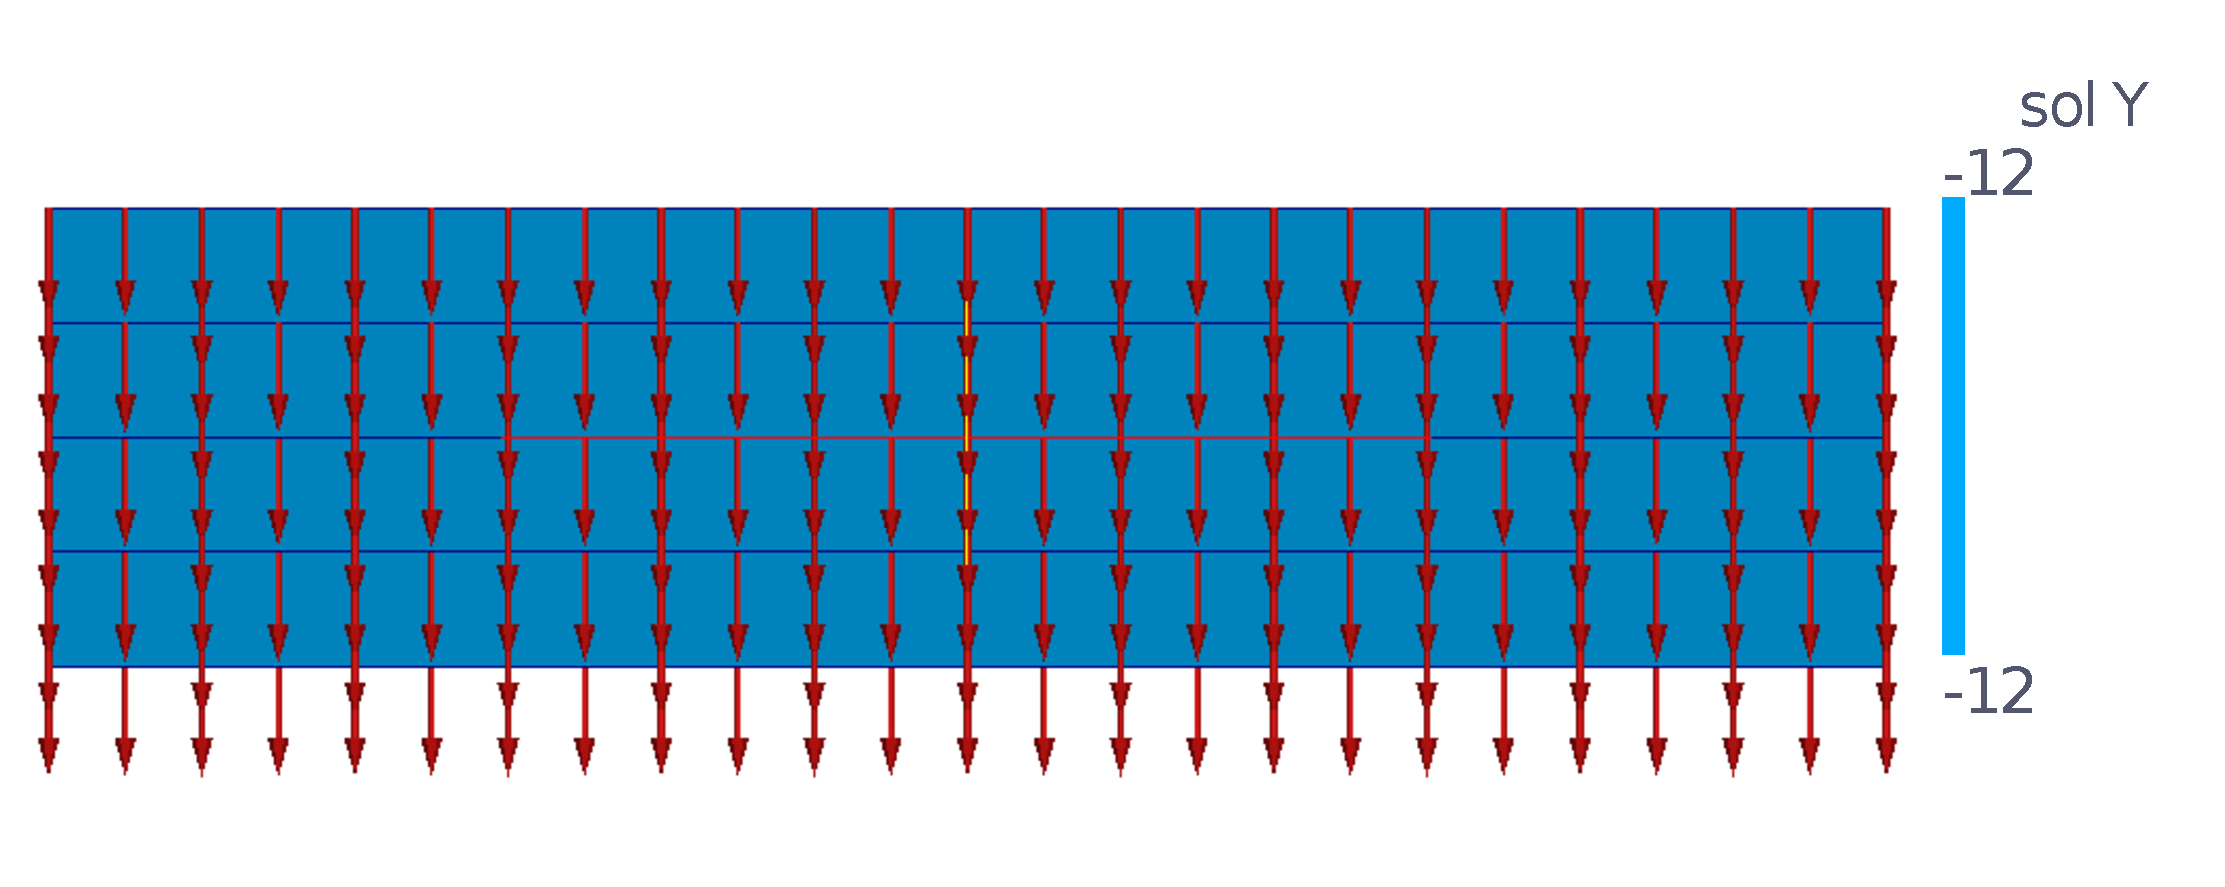
\includegraphics[scale=0.3]{./img/capacitor.pdf}
\caption{Solution of electric field in parallel plate capacitor.}
\label{fig:capacitor}
\end{figure}

It can be seen that the lines don't change in either magnitude or direction, and go from the charged plate wit potential $V_0$ to the bottom plate as expected.

This test showed that the routines for assembling stiffness matrices are capable of continuing a simple field over a distance between to boundaries.

The script for producing this simulation and the necessary input files can be seen in the 
\href{https://github.com/bebopsan/peyeQM/tree/Depuration/Lib/OOPyQM/Examples/Capacitor}{\textit{repository}.}

\subsubsection{Charged cylinder}

The next field problem to solve in order to test PeyeQM was one with circular geometry. The solution for the field due to a point charge or a charged cylinder was used to compare the precision of the method for representing fields with two components.

Gauss law \ref{eq:Gauss} in spherical coordinates, assuming a homogeneous medium with scalar permittivity is:

\begin{equation}
\epsilon \int_S \mathbf{E}\cdot d\mathbf{S} = \int_V \rho dV
\end{equation}

Where $\int_V \rho dV = q$ is the charge of the particle. If that charge is distributed uniformly, then there are no preferred directions and the electric field must be radial \cite{Cheng1993} and have constant intensity over spherical shells. So for an arbitrary 
spherical shell of radius $r$:

\begin{align*}
&\epsilon \mathbf{E} \int_{\theta}\int_{\phi} r^2 sin(\theta) d \phi = q \\
& \mathbf{E}_r(r) = \frac{q}{4\pi \epsilon r^2} \hat{r}
\end{align*}
Now, this has to be transformed into Cartesian coordinates in order to input boundary conditions. If we consider $r$ as the magnitude of vector $\vec{r}$ in the unitary direction $\hat{r}$ then we can transform it to a linear combination of unitary vectors $\hat{x}$ and $\hat{y}$ by the following:
\begin{equation}
\vec{r} = r cos(\theta) \hat{x} + r sin(\theta) \hat{y}
\end{equation}
And by trigonometry we know that $cos(\theta) =\dfrac{x}{r}$ and $sin(\theta)=\dfrac{y}{r}$. Making the necessary substitutions we get to:

\begin{equation}
\mathbf{E}_r(r) = \mathbf{E}_x(x,y) + \mathbf{E}_y(x,y) = \frac{qx}{4\pi \epsilon \sqrt{\left(x^2+y^2\right)}^3} \hat{x}+\frac{qy}{4\pi \epsilon \sqrt{\left(x^2+y^2\right)}^3} \hat{y}
\end{equation}
So, a plot the solution after simulating should match a representation of this analytic result. We initially proposed a model where the charged cylinder or point source is modeled as a \href{https://github.com/bebopsan/peyeQM/tree/
Depuration/Lib/OOPyQM/Examples/Whole\%20cylinder}{whole circle inside a square domain}, the results of the simulation ( figure \ref{fig:whole_cylinder}) showed that for this kind of problem where the field decays in the form $\dfrac{1}{r^2}$ it was better to use finer meshes and take advantage of symmetries to reduce the computational cost. 
Taking just an eight of the model, and reshaping the outer boundary to a circle improved the quality of the elements and allowed us to use a finer mesh. figure \ref{fig:eight_of_cylinder} shows the $y$ and $x$ components of the field as well as the error between the simulation and the analytic solution.
For the simulation factor $\dfrac{q}{2\pi \epsilon}$ has been normalized to 1, and the mesh was done done using 1996 QUAD8 elements with 5525 nodes, thus 11050 degrees of freedom. As a comparison, the simulation of the whole circle involved 2432 elements and 7040 nodes with 14080 degrees of freedom, but it solved for a domain that was eight times bigger.


\begin{figure}
\centering
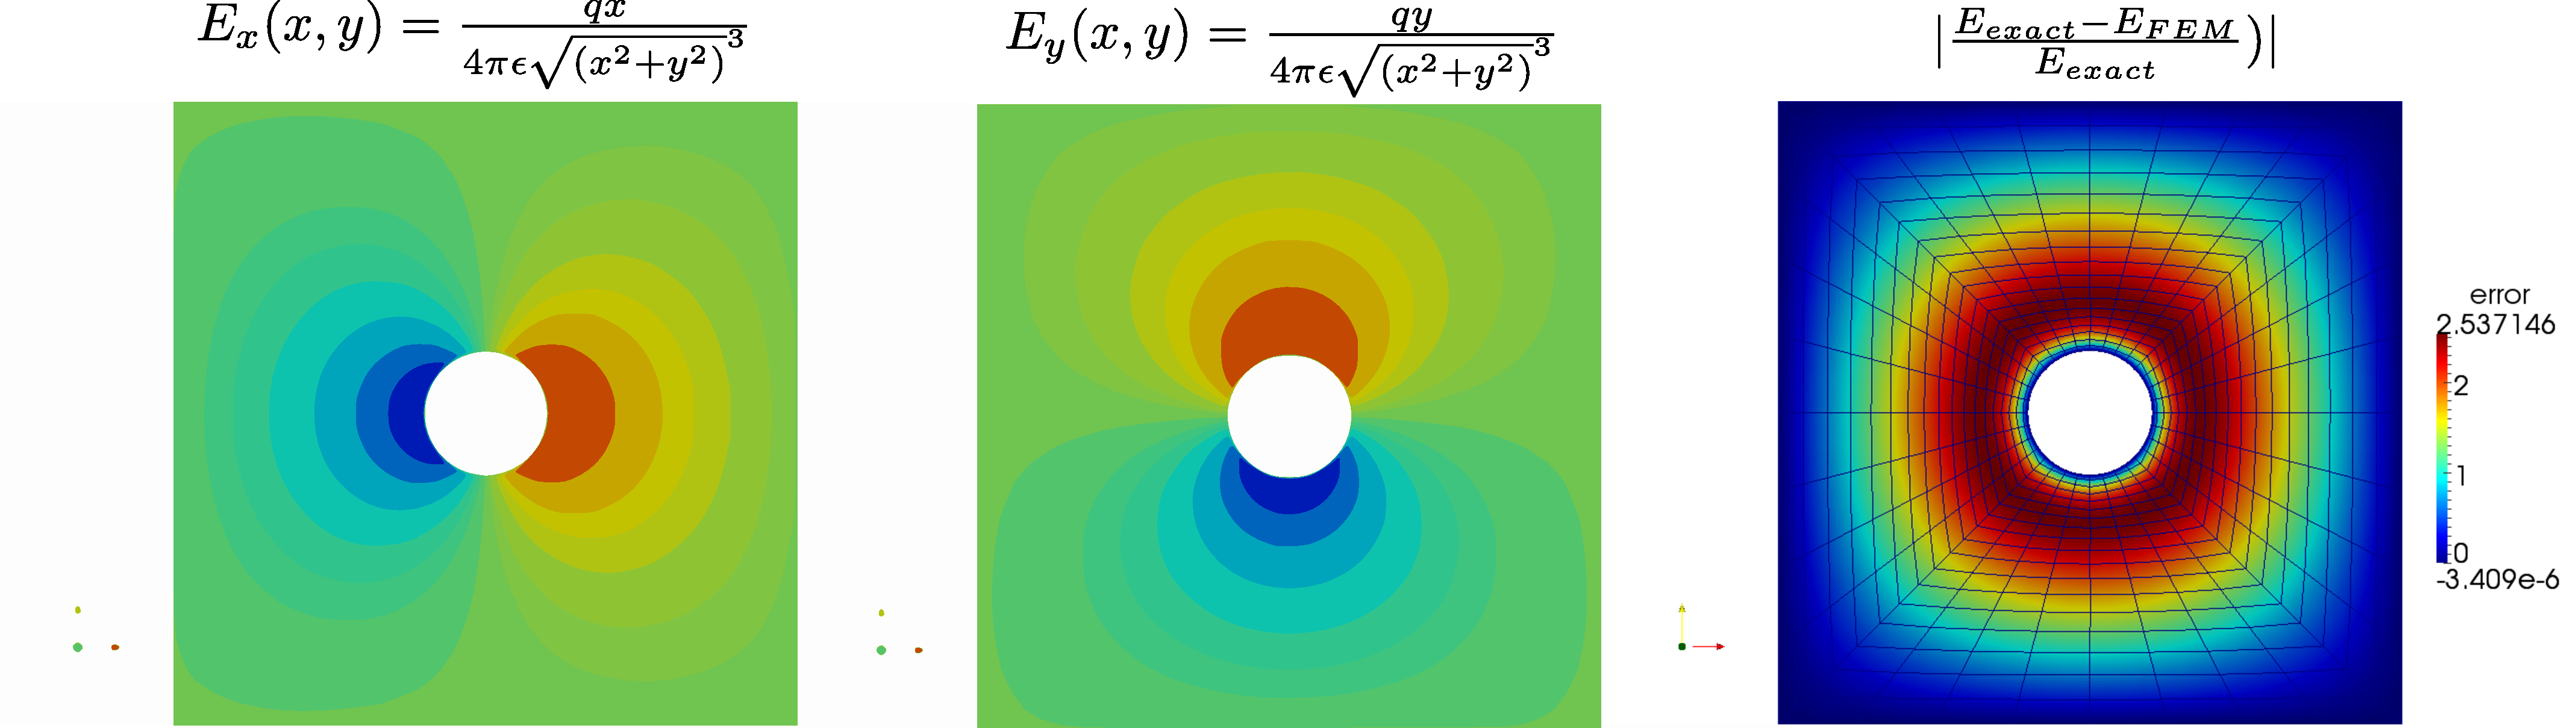
\includegraphics[scale=0.2]{./img/charged_cylinder_inside_rectangle.pdf}
\caption{Whole simulation of Electric field due to a charged cylinder. Left, Numerical result for the $x$ component of the field. Middle, $x$ component of the solution, and, right, mesh and error calculated between analytic formula and results.}
\label{fig:whole_cylinder}
\end{figure}
 
\begin{figure}
\centering
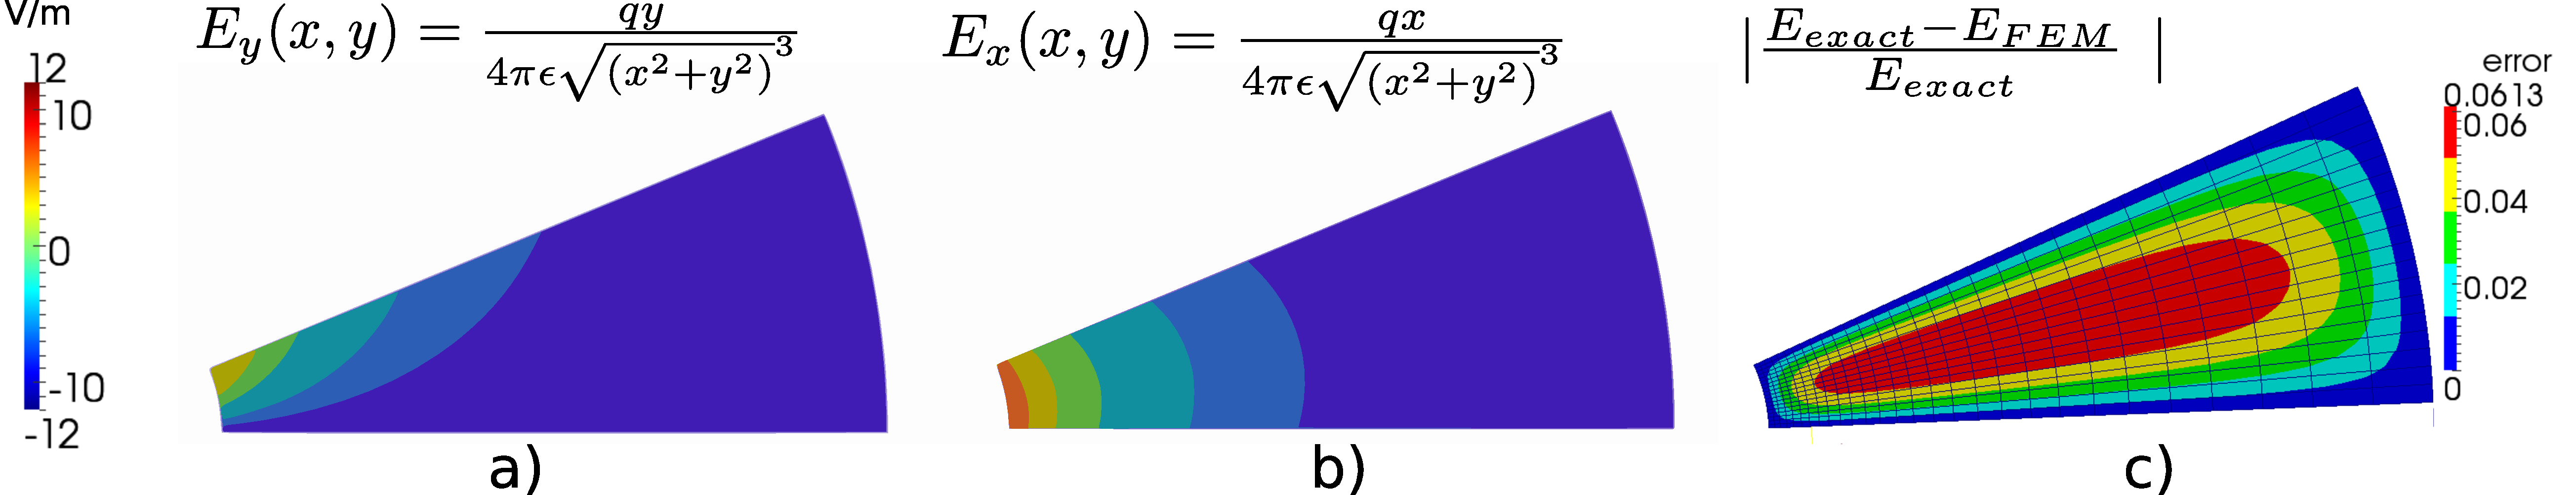
\includegraphics[scale=0.2]{./img/Eight_of_cylinder.pdf}
\caption{Segment of the simulation for Electric field due to a charged cylinder. a) Numerical result for the $y$ component of the field, b) x component of the solution, c) Mesh and error calculated between analytic formula and results.}
\label{fig:eight_of_cylinder}
\end{figure}

\subsubsection{Electric Dipole, two charged spheres.}

A similar simulation was performed using two semicircular surfaces, taking advantage of inversion symmetry along $x$ axis. Boundary conditions are Dirichlet conditions over the circles and the rectangular boundaries on top, and Neumann conditions set to 0 on bottom lines.  The analytic solution is simply the overlapping of the field due to charge 1 and charge 2, having one of them centered in the origin, and the other displaced by a distance $d$. The field everywhere can be expressed as: 

\begin{align}
&\mathbf{E}_1(x,y)=x\left(x^2+y^2\right)^{-\frac{3}{2}}\hat{x} + y\left(x^2+y^2\right)^{\frac{3}{2}}\hat{y}\\ 
&\mathbf{E}_2(x,y)=-(x-4)\left((x-4)^2+y^2\right)^{-\frac{3}{2}} \hat{x}-y\left((x-4)^2+y^2\right)^{\frac{3}{2}}\hat{y}\\
&\mathbf{E}_x = \left[ x\left(x^2+y^2\right)^{-\frac{3}{2}} -(x-4)\left((x-4)^2+y^2\right)^{-\frac{3}{2}}\right] \hat{x}\\
&\mathbf{E}_y =\left[ y\left(x^2+y^2\right)^{\frac{3}{2}} -y\left((x-4)^2+y^2\right)^{\frac{3}{2}}\right]\hat{y}
\end{align}

Where again $\dfrac{q}{2\pi \epsilon} = 1$ for the left charged circle and $-1$ for the one on the right at a distance $d=4$. Figure \ref{fig:two_cylinders} shows components $x$ and $y$ of the resulting field as obtained from the FE solver. The direction of the field lines can be observed by means of arrow glyphs in figure \ref{fig:two_cylinders_glyph}, where field lines go outwards in the positively charged cylinder and inwards in the negative.
In the same way as before, a comparison between analytic and numerical solutions was performed (figure \ref{fig:two_cylinders_error}) and error appeared to be magnified in the region between cylinders. This value keeps being higher than expected, and different meshing schemes were tested in order to improve accuracy. Less error was observed using adaptative meshing methods than structured grids. The current mesh for this simulation has 510 elements and 1622 degrees of freedom, a future simulation is proposed with finer meshes using a PC with bigger RAM.

\begin{figure}
\centering
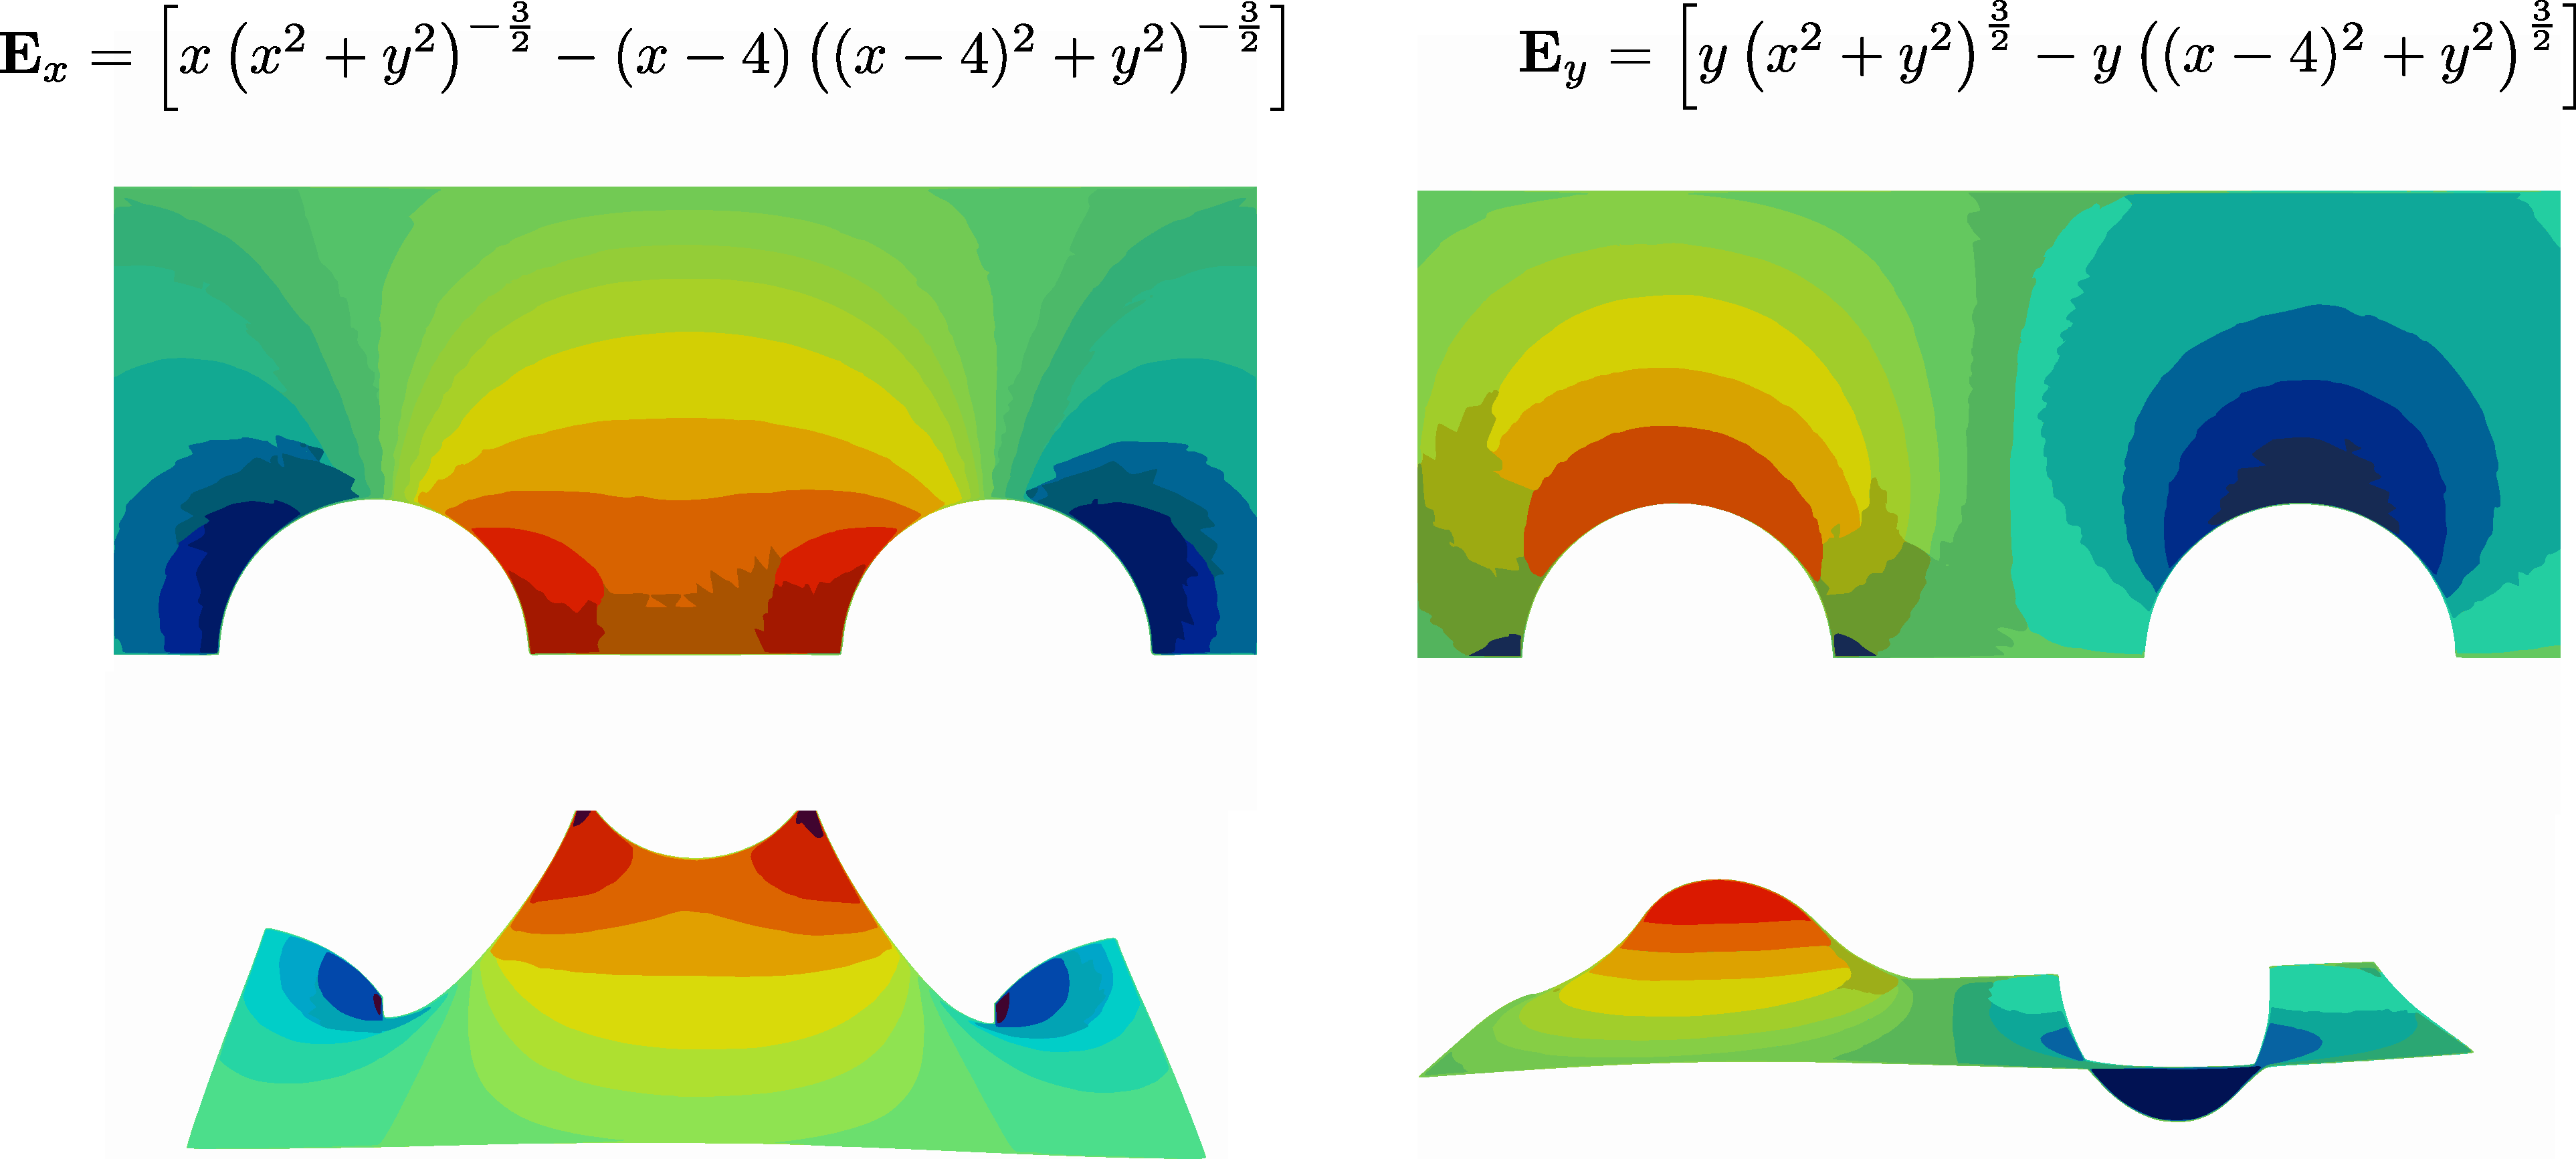
\includegraphics[scale=0.2]{./img/two_cylinders.pdf}
\caption{Components of the electric field after simulating a problem of two cylinders with opposite charges.}
\label{fig:two_cylinders}
\end{figure}

\begin{figure}
\centering
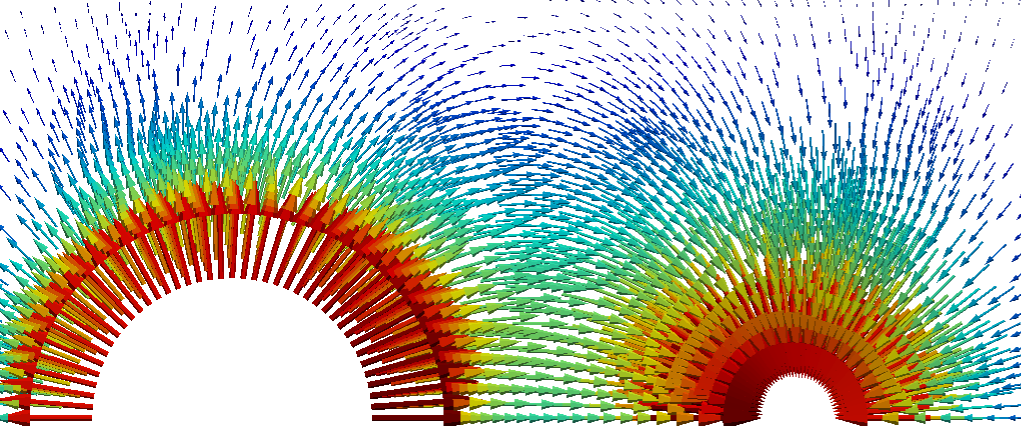
\includegraphics[scale=0.5]{./img/two_cylinders_Gliphs}
\caption{Arrow glyphs of the solution for the dipole problem. Lenght and color of the arrow indicate magnitude of the field. As expected, the field points from the positively charged cylinder to the negative.}
\label{fig:two_cylinders_glyph}
\end{figure}

\begin{figure}
\centering
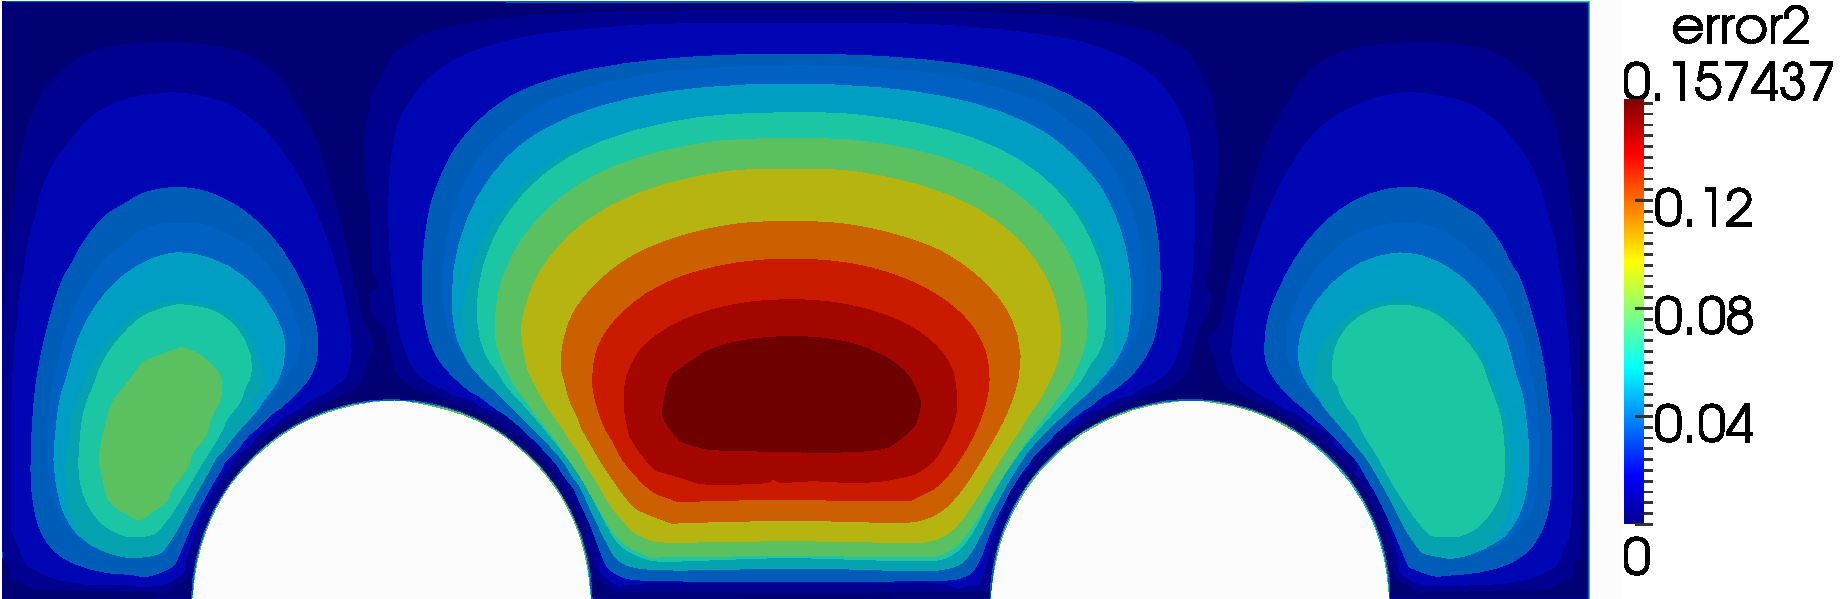
\includegraphics[scale=0.4]{./img/two_cylinders_error.pdf}
\caption{Error calculation of simulation against exact solution. The method reproduces the nature of the problem, but a finer mesh is needed to obtain precise results.}
\label{fig:two_cylinders_error}
\end{figure}

\section{Harmonic benchmark tests}
The second section regards solutions of eigenvalue problems, either for closed domains or infinite and periodic ones. The first part will deal with simulation of resonant modes in wave guides, and the second with free waves and periodic crystals.

\subsection{Eigenvalues and modes in waveguides}

Ideal wave guides can be modelled by a source-less version of the wave equation for time harmonic fields \ref{eq:E-wave-harmonic} in arbitrary 2D domains closed by a metallic boundary that guarantees Dirichlet condition $\mathbf{E} = 0\quad at\quad \Gamma$. This problem is relevant in electromagnetism and telecommunications because it is the principle behind many applications such as data transmission in fiber optics, and microwaves. Here, the 2D domain represents a cross section of a metallic structure that guides waves along its axis. We are particularly interested in knowing two things:
\begin{enumerate}
\item The modes or wave functions that are solution to the equation for a particular shape.
\item The frequencies associated to those modes or shapes. 
\end{enumerate}
And will start by introducing the analytic solution behind simple wave guides such as rectangular and circular guides.

\subsubsection{Rectangular waveguides} 

In transverse magnetic fields (TM) that travel inside a waveguide whose axis is over $z$, we have $\mathbf{H}_z = 0$ and solve for $\mathbf{E}$ components. 
Solutions of equation \ref{eq:E-wave-harmonic2} where the medium inside the wave guide is a perfect dielectric, and  for eigenvalues $\vec{k}^2 = \omega^2\mu\epsilon$ is a lengthy but straightforward process that involves separation of variables and use of boundary conditions:
\begin{align}
&\mathbf{E}_x = 0 \quad for \quad y=0,\ 0<x<a\\
&\mathbf{E}_x = 0 \quad for \quad y=b,\ 0<x<a\\
&\mathbf{E}_y = 0 \quad for \quad x=0,\ 0<y<b\\
&\mathbf{E}_y = 0 \quad for \quad x=a,\ 0<y<b
\end{align}

A description of the solution process is left for the reader to look up in references such as Rao  \cite{Rao2004} or Jianming \cite{Jin2010}. What is found in the process is that only certain discrete frequencies are allowed inside the waveguide, and they are given by:

\begin{equation}
\omega_{n,m} = \frac{1}{\sqrt{\mu\epsilon}}\sqrt{\left(\frac{m\pi}{a}\right)^2+\left(\frac{n\pi}{b}\right)^2}
\qquad m,n = 0,1,2,... \quad (m=n\neq0)
\label{eq:eig_vals_sqare_waveguide}
\end{equation}
Where $\omega$ is indexed by integers $n,m$ and the trivial solution $\omega = 0$ is excluded. $a$ is the width of the rectangular cross section and $b$ is its height.
The wave functions that are solution to this eigenproblem for each component of the field are in the following general form:

\begin{align}
&\mathbf{E}_z = A\sin{\dfrac{m\pi x}{a}}\sin{\dfrac{n\pi x}{b}}e^{\mp jk_zz} \label{eq:Ez_mag}\\
&\mathbf{E}_x =\mp jB\dfrac{m\pi}{a}\cos{\dfrac{m\pi x}{a}}\sin{\dfrac{n\pi x}{b}}e^{\mp jk_zz}\\
&\mathbf{E}_y =\mp jC\dfrac{n\pi}{b}\sin{\dfrac{m\pi x}{a}}\cos{\dfrac{n\pi x}{b}}e^{\mp jk_zz}
\end{align}

For our comparisons we will only look at how closely the shapes of the simulated solution represent $\mathbf{E}$ in \ref{eq:Ez_mag}, and how similar are the analýtic and numeric  natural frequencies of the guide $\omega$.



